% 20120511-132418-132718
% A-6.8/W31.3

\section{A-6.8/W31.3 - 170 krpm}
\label[secinapp]{sec:awp-exp-details-A-6.8/W31.3}

This test has been performed on May 11\th{} 2012, between 13:24:18 and
13:27:18.

\begin{figure}[htbp]
  \centering
  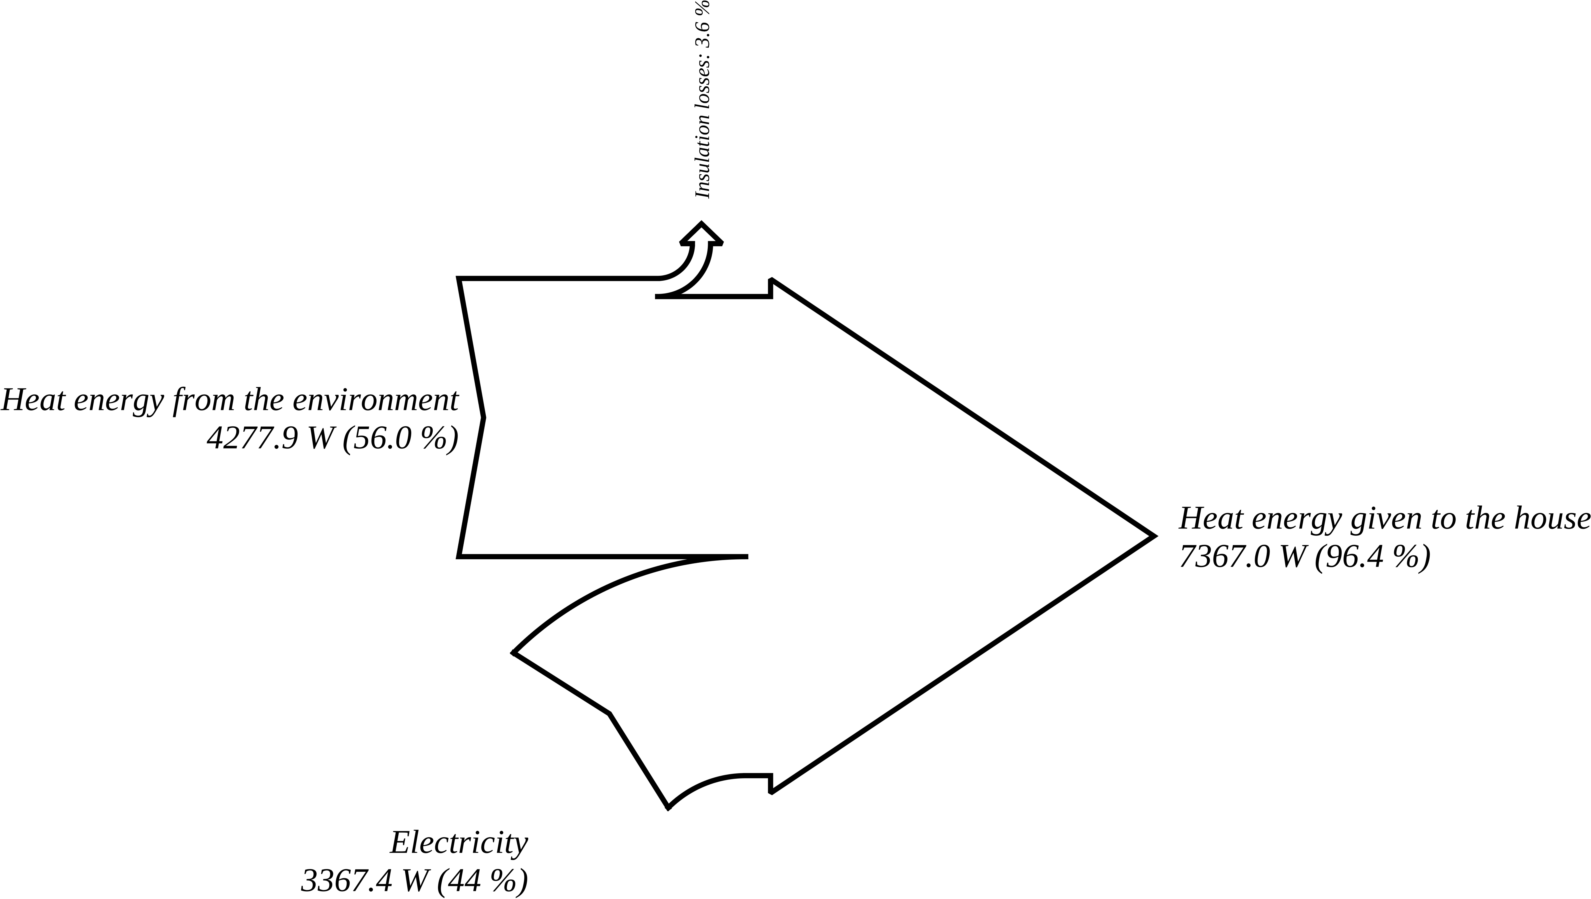
\includegraphics[width=0.7\textwidth]{awp-energy-sankey-awp-20120511-132418-132718}
  \caption{A-6.8/W31.3 -- Sankey diagram for heat pump energy balance (internal frontier)}
  \label{fig:awp-A-6.8/W31.3-sankey-energy}
\end{figure}


\begin{figure}[htbp]
  \centering
  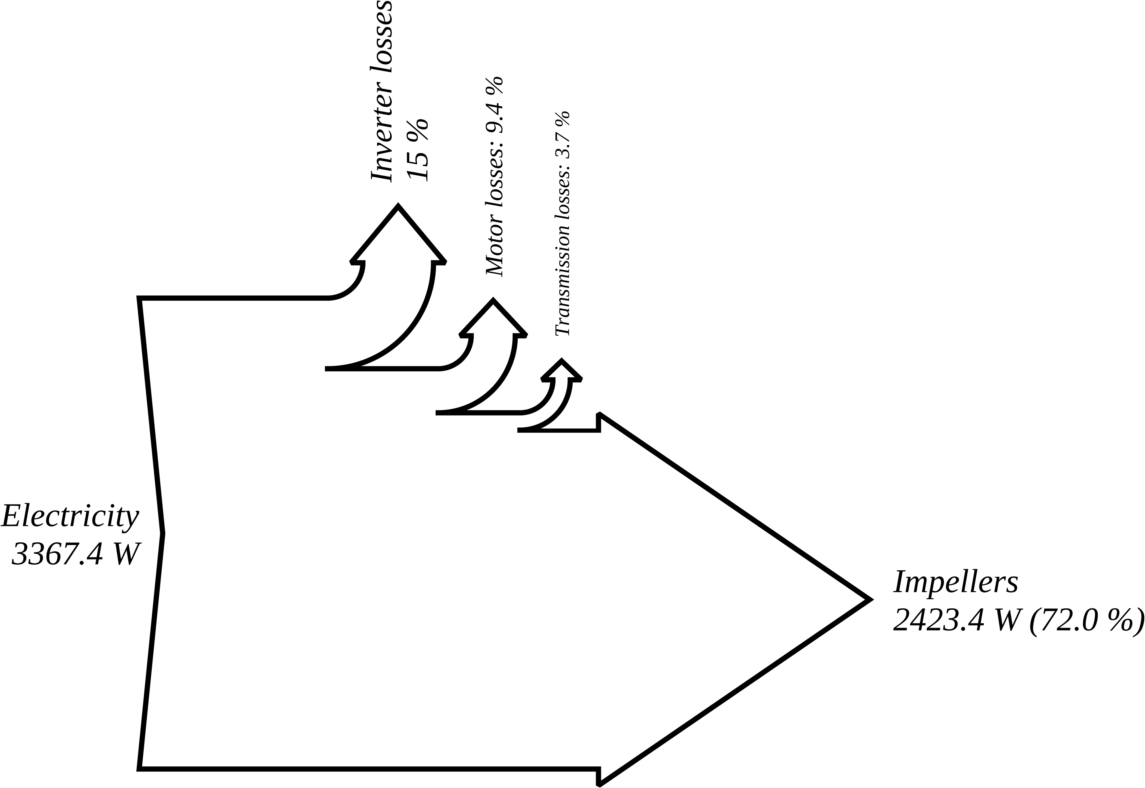
\includegraphics[width=0.7\textwidth]{awp-energy-sankey-cp-20120511-132418-132718}
  \caption{A-6.8/W31.3 -- Sankey diagram for the compressor unit energy balance}
  \label{fig:awp-A-6.8/W31.3-sankey-cp}
\end{figure}

\begin{figure}[htbp]
  \centering
  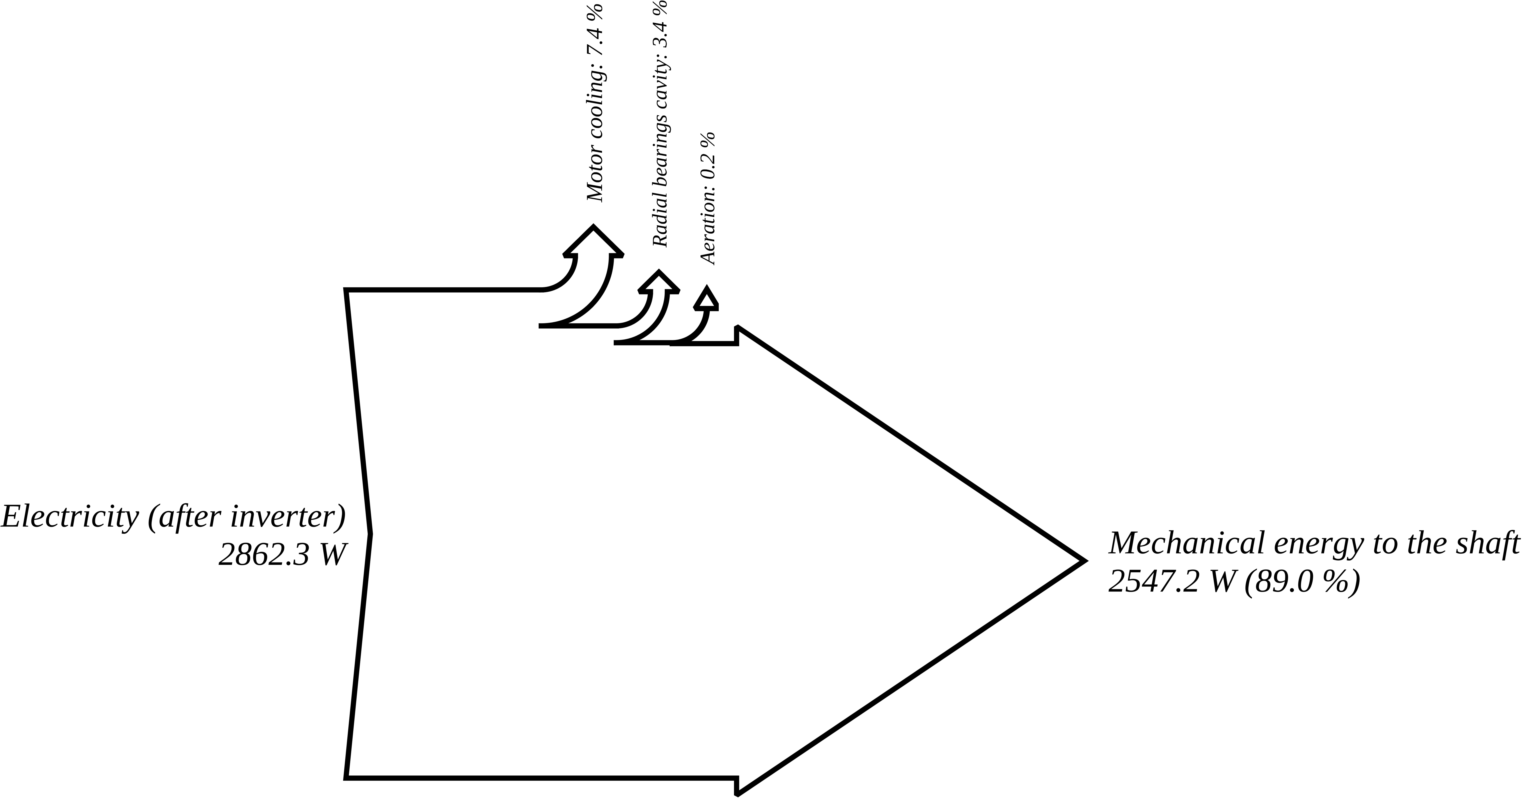
\includegraphics[width=0.7\textwidth]{awp-energy-sankey-motor-20120511-132418-132718}
  \caption{A-6.8/W31.3 -- Sankey diagram for the motor energy balance}
  \label{fig:awp-A-6.8/W31.3-sankey-motor}
\end{figure}

\begin{table}[htbp]
    \footnotesize
    \begin{center}
    \begin{tabular}{llllll}
\toprule
Name & Value / \% & Name & Value / \% & Name & Value / - \\
\midrule
$\eta_{heatpump}$ & $ \num{26.3} \pm \num{0.7} $ & $\eta_{mot}$ & $ \num{88.9} \pm \num{0.2} $ & $\epsilon_h$ & $ \num{2.19} \pm \num{0.04} $\\
$\eta_{cp1}$ & $ \num{59} \pm \num{40} $ & $\eta_{cp2}$ &$ \num{81} \pm \num{19} $ & $\pi_1$ & $ \num{2.848} \pm \num{0.005} $\\
$\eta_{cp1,\,imp}$ & $ \num{59} \pm \num{40} $ & $\eta_{cp2,\,imp}$ & $ \num{83} \pm \num{17} $ & $\pi_2$ & $ \num{2.703} \pm \num{0.002} $\\
$\eta_{cd}$ & $ \num{94} \pm \num{3} $ & $\eta_{ev}$ & $ \num{17} \pm \num{17} $ & $\pi_{1,\,theory}$ & $ \num{3.3} \pm \num{0.2} $\\
$\eta_{trans}$ & $ \num{95.14} \pm \num{0.02} $ & $\eta_{sc}$ & $ \num{1} \pm \num{1} $ & $\pi_{2,\,theory}$ & $ \num{2.672} \pm \num{0.001} $\\
$\eta_{s,\,cp1}$ & $ \num{88} \pm \num{12} $ & $\eta_{s,\,cp2}$ & $ \num{89} \pm \num{11} $ & $\eta_{mot}$ & $\underline{88.99}$ \%\\
$\eta_{s,\,cp1,\,ext}$ & $ \num{90} \pm \num{10} $ & $\eta_{s,\,cp2,\,ext}$ & $ \num{82} \pm \num{19} $ & $\eta_{radial}$ & $ \num{98.21} \pm \num{0.02} $ \%\\
$\eta_{s,\,cp1,\,theory}$ & $ \num{78} \pm \num{2} $ & $\eta_{s,\,cp2,\,theory}$ & $ \num{79.482} \pm \num{0.002} $ & $\eta_{axial}$ & $ \num{96.88} \pm \num{0.02} $ \%\\
\bottomrule
\end{tabular}

  \end{center}
  \caption{A-6.8/W31.3 -- Performance indicators}
\end{table}

\begin{table}[htbp]
  \footnotesize
  \begin{center}
    \begin{tabular}{cccccc}
\toprule
Component & Location & P / \si{\bar} & T / \si{\degreeCelsius} & h / \si{\kilo\joule\per\kilo\gram} & s / \si{\kilo\joule\per\kilo\gram\per\kelvin}\\
\midrule
\multirow{2}{*}{1} & inlet & $ \num{1.073} \pm \num{0.002} $ & $ \num{-18} \pm \num{7} $ & $ \num{388.678} \pm \num{0.007} $ & $ \num{1.77} \pm \num{0.02} $\\
& outlet & $ \num{3.058} \pm \num{0.002} $ & $ \num{33.7} \pm \num{0.6} $ & $ \num{428.3668} \pm \num{5e-04} $ & $ \num{1.827} \pm \num{0.003} $\\
\midrule
\multirow{2}{*}{2} & inlet & $\pmb{ \num{3.058} \pm \num{0.002} }$ & $\pmb{ \num{8.683} \pm \num{0.007} }$ & $ \num{406.015796} \pm \num{7e-06} $ & $ \num{1.75057} \pm \num{8e-05} $\\
& outlet & $\pmb{ \num{8.265} \pm \num{0.002} }$ & $\pmb{ \num{50.761} \pm \num{0.007} }$ & $ \num{435.116938} \pm \num{7e-06} $ & $ \num{1.77439} \pm \num{5e-05} $\\
\midrule
\multirow{2}{*}{3} & inlet & $\pmb{ \num{8.148} \pm \num{0.002} }$ & $\pmb{ \num{44.228} \pm \num{0.006} }$ & $ \num{428.645708} \pm \num{6e-06} $ & $ \num{1.75520} \pm \num{4e-05} $\\
& outlet & $\pmb{ \num{7.947} \pm \num{0.002} }$ & $\pmb{ \num{29.426} \pm \num{0.006} }$ & $ \num{240.892167} \pm \num{6e-06} $ & $ \num{1.14069} \pm \num{3e-05} $\\
\midrule
\multirow{2}{*}{4} & inlet & $ \num{1.776} \pm \num{0.002} $ & $ \num{-13.0} \pm \num{0.8} $ & $ \num{221.2280} \pm \num{8e-04} $ & $ \num{1.084} \pm \num{0.003} $\\
& outlet & $\pmb{ \num{1.670} \pm \num{0.002} }$ & $\pmb{ \num{-14.176} \pm \num{0.006} }$ & $ \num{390.214173} \pm \num{6e-06} $ & $ \num{1.7379} \pm \num{1e-04} $\\
\midrule
\multirow{2}{*}{5} & inlet & $ \num{7.947} \pm \num{0.002} $ & $ \num{29.43} \pm \num{0.04} $ & $ \num{240.89217} \pm \num{4e-05} $ & $ \num{1.1407} \pm \num{2e-04} $\\
& outlet & $ \num{3.058} \pm \num{0.002} $ & $ \num{1.2} \pm \num{0.5} $ & $ \num{240.8922} \pm \num{5e-04} $ & $ \num{1.149} \pm \num{0.002} $\\
\midrule
\multirow{2}{*}{6} & inlet & $ \num{3.058} \pm \num{0.002} $ & $ \num{-5} \pm \num{11} $ & $ \num{193.72} \pm \num{0.02} $ & $ \num{0.98} \pm \num{0.06} $\\
& outlet & $ \num{1.896} \pm \num{0.002} $ & $ \num{-11.4} \pm \num{0.8} $ & $ \num{193.7184} \pm \num{8e-04} $ & $ \num{0.978} \pm \num{0.004} $\\
\midrule
\multirow{2}{*}{7} & inlet & $ \num{1.896} \pm \num{0.002} $ & $ \num{-11.4} \pm \num{0.8} $ & $ \num{240.8922} \pm \num{8e-04} $ & $ \num{1.158} \pm \num{0.003} $\\
& outlet & $ \num{1.896} \pm \num{0.002} $ & $ \num{-11.4} \pm \num{0.8} $ & $ \num{281.5177} \pm \num{8e-04} $ & $ \num{1.313} \pm \num{0.002} $\\
\midrule
\multirow{2}{*}{8} & inlet & $\pmb{ \num{3.058} \pm \num{0.002} }$ & $\pmb{ \num{1.201} \pm \num{0.007} }$ & $ \num{399.302716} \pm \num{7e-06} $ & $ \num{1.72643} \pm \num{2e-05} $\\
& outlet & $ \num{3.06} \pm \num{0.06} $ & $ \num{1.2} \pm \num{0.5} $ & $ \num{201.6155} \pm \num{5e-04} $ & $ \num{1.006} \pm \num{0.003} $\\
\midrule
\multirow{2}{*}{9} & inlet & $\pmb{ \num{1.896} \pm \num{0.002} }$ & $\pmb{ \num{-11.422} \pm \num{0.006} }$ & $ \num{221.228042} \pm \num{6e-06} $ & $ \num{1.08263} \pm \num{8e-05} $\\
& outlet & $ \num{1.776} \pm \num{0.002} $ & $ \num{-13.0} \pm \num{0.8} $ & $ \num{221.2280} \pm \num{8e-04} $ & $ \num{1.084} \pm \num{0.003} $\\
\midrule
\multirow{2}{*}{10} & inlet & $ \num{8.265} \pm \num{0.002} $ & $ \num{50.8} \pm \num{0.3} $ & $ \num{435.1169} \pm \num{3e-04} $ & $ \num{1.774} \pm \num{0.001} $\\
& outlet & $ \num{3.058} \pm \num{0.002} $ & $ \num{149} \pm \num{101} $ & $ \num{540.6} \pm \num{0.2} $ & $ \num{2.1} \pm \num{0.3} $\\
\midrule
\multirow{2}{*}{11} & inlet & $ \num{1.073} \pm \num{0.002} $ & $ \num{95} \pm \num{43} $ & $ \num{487.85} \pm \num{0.05} $ & $ \num{2.1} \pm \num{0.1} $\\
& outlet & $ \num{1.073} \pm \num{0.002} $ & $ \num{127} \pm \num{58} $ & $ \num{519.46} \pm \num{0.06} $ & $ \num{2.2} \pm \num{0.2} $\\
\midrule
\multirow{2}{*}{12} & inlet & $ \num{2.500} \pm \num{0.002} $ & $ \num{20} \pm \num{24} $ & $ \num{416.89} \pm \num{0.03} $ & $ \num{1.80} \pm \num{0.07} $\\
& outlet & $ \num{2.500} \pm \num{0.002} $ & $ \num{44} \pm \num{37} $ & $ \num{438.58} \pm \num{0.04} $ & $ \num{1.9} \pm \num{0.1} $\\
\midrule
\multirow{2}{*}{13} & inlet & $ \num{2.491} \pm \num{0.002} $ & $ \num{14.5} \pm \num{0.7} $ & $ \num{412.4779} \pm \num{7e-04} $ & $ \num{1.789} \pm \num{0.004} $\\
& outlet & $ \num{2.491} \pm \num{0.002} $ & $ \num{20} \pm \num{25} $ & $ \num{417.74} \pm \num{0.03} $ & $ \num{1.81} \pm \num{0.08} $\\
\midrule
\multirow{2}{*}{15} & inlet & & $\pmb{ \num{26.487} \pm \num{0.006} }$ & \multicolumn{2}{l}{Cp = $ \num{4180.476} \pm \num{0.002} $ \si{\joule\per\kilo\gram\per\kelvin}}\\
& outlet & & $\pmb{ \num{31.252} \pm \num{0.006} }$ & \multicolumn{2}{l}{Cp = $ \num{4179.3369} \pm \num{9e-04} $ \si{\joule\per\kilo\gram\per\kelvin}}\\
\midrule
\multirow{2}{*}{16} & inlet & & $\pmb{ \num{-6.775} \pm \num{0.006} }$ & & \\
& outlet & & $\pmb{ \num{-9.932} \pm \num{0.006} }$ & & \\
\midrule
\multirow{2}{*}{18} & inlet & $ \num{1.670} \pm \num{0.002} $ & $ \num{-14.2} \pm \num{0.4} $ & $ \num{390.2142} \pm \num{4e-04} $ & $ \num{1.738} \pm \num{0.003} $\\
& outlet & $\pmb{ \num{1.073} \pm \num{0.002} }$ & $\pmb{ \num{-24.77} \pm \num{0.01} }$ & $ \num{383.60197} \pm \num{1e-05} $ & $ \num{1.7460} \pm \num{2e-04} $\\
\midrule
\multirow{2}{*}{19} & inlet & $ \num{3.058} \pm \num{0.002} $ & $ \num{1.2} \pm \num{0.5} $ & $ \num{201.6155} \pm \num{5e-04} $ & $ \num{1.006} \pm \num{0.003} $\\
& outlet & $ \num{3.058} \pm \num{0.002} $ & $ \num{-5} \pm \num{11} $ & $ \num{193.72} \pm \num{0.02} $ & $ \num{0.98} \pm \num{0.06} $\\
\midrule
\multirow{2}{*}{20} & inlet & $ \num{8.265} \pm \num{0.002} $ & $ \num{50.8} \pm \num{0.3} $ & $ \num{435.1169} \pm \num{3e-04} $ & $ \num{1.774} \pm \num{0.001} $\\
& outlet & $ \num{8.148} \pm \num{0.002} $ & $ \num{44.2} \pm \num{0.3} $ & $ \num{428.6457} \pm \num{3e-04} $ & $ \num{1.755} \pm \num{0.001} $\\
\midrule
\multirow{2}{*}{21} & inlet & $ \num{2.491} \pm \num{0.002} $ & $ \num{14.5} \pm \num{0.7} $ & $ \num{412.4779} \pm \num{7e-04} $ & $ \num{1.789} \pm \num{0.004} $\\
& outlet & $\pmb{ \num{2.500} \pm \num{0.002} }$ & $\pmb{ \num{14.472} \pm \num{0.007} }$ & $ \num{412.457806} \pm \num{7e-06} $ & $ \num{1.78846} \pm \num{8e-05} $\\
\midrule
\multirow{2}{*}{22} & inlet & $ \num{1.073} \pm \num{0.002} $ & $ \num{-20} \pm \num{5} $ & $ \num{387.658} \pm \num{0.005} $ & $ \num{1.76} \pm \num{0.02} $\\
& outlet & $\pmb{ \num{1.073} \pm \num{0.002} }$ & $\pmb{ \num{-19.689} \pm \num{0.007} }$ & $ \num{387.657800} \pm \num{7e-06} $ & $ \num{1.7622} \pm \num{2e-04} $\\
\midrule
\multirow{2}{*}{23} & inlet & $ \num{1.073} \pm \num{0.002} $ & $ \num{127} \pm \num{58} $ & $ \num{519.46} \pm \num{0.06} $ & $ \num{2.2} \pm \num{0.2} $\\
& outlet & $ \num{1.073} \pm \num{0.002} $ & $ \num{150} \pm \num{65} $ & $ \num{543.18} \pm \num{0.07} $ & $ \num{2.2} \pm \num{0.2} $\\
\midrule
\multirow{2}{*}{24} & inlet & $ \num{1.073} \pm \num{0.002} $ & $ \num{41} \pm \num{38} $ & $ \num{438.58} \pm \num{0.04} $ & $ \num{1.9} \pm \num{0.1} $\\
& outlet & $ \num{1.073} \pm \num{0.002} $ & $ \num{95} \pm \num{43} $ & $ \num{487.85} \pm \num{0.05} $ & $ \num{2.1} \pm \num{0.1} $\\
\midrule
\multirow{2}{*}{25} & inlet & $ \num{3.058} \pm \num{0.002} $ & $ \num{34} \pm \num{28} $ & $ \num{429.02} \pm \num{0.03} $ & $ \num{1.83} \pm \num{0.08} $\\
& outlet & $\pmb{ \num{3.058} \pm \num{0.002} }$ & $\pmb{ \num{34.389} \pm \num{0.007} }$ & $ \num{429.015934} \pm \num{7e-06} $ & $ \num{1.82866} \pm \num{7e-05} $\\
\midrule
\multirow{2}{*}{26} & inlet & $ \num{8.265} \pm \num{0.002} $ & $ \num{50.8} \pm \num{0.3} $ & $ \num{435.1169} \pm \num{3e-04} $ & $ \num{1.774} \pm \num{0.001} $\\
& outlet & $\pmb{ \num{2.491} \pm \num{0.002} }$ & $\pmb{ \num{14.472} \pm \num{0.007} }$ & $ \num{412.477899} \pm \num{7e-06} $ & $ \num{1.78880} \pm \num{8e-05} $\\
\midrule
\multirow{2}{*}{27} & inlet & $ \num{3.058} \pm \num{0.002} $ & $ \num{33.7} \pm \num{0.3} $ & $ \num{428.3674} \pm \num{3e-04} $ & $ \num{1.827} \pm \num{0.002} $\\
& outlet & $ \num{3.058} \pm \num{0.002} $ & $ \num{33.7} \pm \num{0.3} $ & $ \num{428.3674} \pm \num{3e-04} $ & $ \num{1.827} \pm \num{0.002} $\\
\midrule
\multirow{2}{*}{28} & inlet & $ \num{3.058} \pm \num{0.002} $ & $ \num{1.2} \pm \num{0.4} $ & $ \num{399.3027} \pm \num{4e-04} $ & $ \num{1.7264} \pm \num{9e-04} $\\
& outlet & $ \num{3.058} \pm \num{0.002} $ & $ \num{8.7} \pm \num{0.4} $ & $ \num{406.0158} \pm \num{4e-04} $ & $ \num{1.751} \pm \num{0.002} $\\
\midrule
\multirow{2}{*}{29} & inlet & $ \num{1.073} \pm \num{0.002} $ & $ \num{-20.6} \pm \num{0.5} $ & $ \num{386.9432} \pm \num{5e-04} $ & $ \num{1.759} \pm \num{0.005} $\\
& outlet & $ \num{1.073} \pm \num{0.002} $ & $ \num{-18} \pm \num{7} $ & $ \num{388.678} \pm \num{0.007} $ & $ \num{1.77} \pm \num{0.02} $\\
\bottomrule
\end{tabular}

  \end{center}
  \caption{A-6.8/W31.3 -- Thermodynamic points of the heat pump cycle}
\end{table}


\begin{table}[htbp]
    \footnotesize
    \begin{center}
    \begin{tabular}{llllll}
\toprule
Name & Value / \si{\gram\per\second} & Name & Value / \si{\gram\per\second} & Name & Value / \si{\gram\per\second} \\
\midrule
$\dot{M}_{1 \rightarrow 25}$ & $ \num{33} \pm \num{2} $ & $\dot{M}_{2 \rightarrow 10}$ & $\underline{0.19}$ & $\dot{M}_{2 \rightarrow 20}$ & $ \num{39.2} \pm \num{0.8} $ \\
$\dot{M}_{2 \rightarrow 26}$ & $\pmb{ \num{1.20} \pm \num{0.06} }$ & $\dot{M}_{3 \rightarrow 5}$ & $ \num{34.0} \pm \num{0.8} $ & $\dot{M}_{3 \rightarrow 7}$ & $\pmb{ \num{5.20} \pm \num{0.09} }$ \\
$\dot{M}_{4 \rightarrow 18}$ & $ \num{32} \pm \num{2} $ & $\dot{M}_{5 \rightarrow 8}$ & $ \num{34.0} \pm \num{0.8} $ & $\dot{M}_{6 \rightarrow 9}$ & $ \num{27} \pm \num{2} $ \\
$\dot{M}_{7 \rightarrow 9}$ & $ \num{5.20} \pm \num{0.09} $ & $\dot{M}_{8 \rightarrow 19}$ & $ \num{27} \pm \num{2} $ & $\dot{M}_{8 \rightarrow 28}$ & $ \num{31} \pm \num{2} $ \\
$\dot{M}_{9 \rightarrow 4}$ & $ \num{32} \pm \num{2} $ & $\dot{M}_{10 \rightarrow 25}$ & $0.19$ & $\dot{M}_{11 \rightarrow 22}$ & $ \num{0.98} \pm \num{0.04} $ \\
$\dot{M}_{11 \rightarrow 23}$ & $ \num{0.22} \pm \num{0.01} $ & $\dot{M}_{12 \rightarrow 24}$ & $ \num{1.20} \pm \num{0.05} $ & $\dot{M}_{13 \rightarrow 12}$ & $ \num{1.01} \pm \num{0.05} $ \\
$\dot{M}_{17 \rightarrow 15}$ & $\pmb{ \num{376} \pm \num{5} }$ & $\dot{M}_{18 \rightarrow 22}$ & $ \num{32} \pm \num{2} $ & $\dot{M}_{19 \rightarrow 6}$ & $ \num{27} \pm \num{2} $ \\
$\dot{M}_{20 \rightarrow 3}$ & $ \num{39.2} \pm \num{0.8} $ & $\dot{M}_{21 \rightarrow 12}$ & $ \num{0.19} \pm \num{0.01} $ & $\dot{M}_{22 \rightarrow 29}$ & $ \num{33} \pm \num{2} $ \\
$\dot{M}_{23 \rightarrow 29}$ & $ \num{0.22} \pm \num{0.01} $ & $\dot{M}_{24 \rightarrow 11}$ & $ \num{1.20} \pm \num{0.05} $ & $\dot{M}_{25 \rightarrow 8}$ & $ \num{24} \pm \num{1} $ \\
$\dot{M}_{25 \rightarrow 27}$ & $ \num{9.4} \pm \num{0.4} $ & $\dot{M}_{26 \rightarrow 13}$ & $ \num{1.01} \pm \num{0.05} $ & $\dot{M}_{26 \rightarrow 21}$ & $ \num{0.19} \pm \num{0.01} $ \\
$\dot{M}_{27 \rightarrow 28}$ & $ \num{9.4} \pm \num{0.4} $ & $\dot{M}_{28 \rightarrow 2}$ & $ \num{41} \pm \num{2} $ & $\dot{M}_{29 \rightarrow 1}$ & $ \num{33} \pm \num{2} $ \\
$\dot{M}_{cp_1}$ & $ \num{33} \pm \num{2} $ & $\dot{M}_{cp_2}$ & $ \num{40.6} \pm \num{0.8} $ \\
\bottomrule
\end{tabular}

  \end{center}
  \caption{A-6.8/W31.3 -- Mass flow rates between the components}
\end{table}

\begin{table}[htbp]
    \footnotesize
    \begin{center}
    \begin{tabular}{llll}
\toprule
Name & Value / $W$ & Name & Value / $W$ \\
\midrule
$\dot{E}_{1 \rightarrow 2}$ & $ \num{1108} \pm \num{1e+03} $ & $\dot{E}_{11 \rightarrow 1}$ & $ \num{2423.4} \pm \num{0.4} $ \\
$\dot{E}_{12 \rightarrow 11}$ & $ \num{2501.5} \pm \num{0.4} $ & $\dot{E}_{13 \rightarrow 12}$ & $ \num{2547.2} \pm \num{0.4} $ \\
$\dot{E}_{14 \rightarrow 13}$ & $ \num{2862.3} \pm \num{0.4} $ & $\dot{E}_{el \rightarrow 14}$ & $\pmb{ \num{3367.4} \pm \num{0.5} }$ \\
$\dot{Y}_{1 \rightarrow 2}$ & $ \num{94} \pm \num{94} $ & $\dot{Y}_{2 \rightarrow 10}$ & $ \num{20} \pm \num{20} $ \\
$\dot{Y}_{3 \rightarrow 15}$ & $ \num{7367} \pm \num{138} $ & $\dot{Y}_{11 \rightarrow 1}$ & $ \num{94} \pm \num{47} $ \\
$\dot{Y}_{11 \rightarrow 23}$ & $ \num{5} \pm \num{3} $ & $\dot{Y}_{11 \rightarrow 24}$ & $ \num{59} \pm \num{59} $ \\
$\dot{Y}_{12 \rightarrow 11}$ & $ \num{118} \pm \num{59} $ & $\dot{Y}_{13 \rightarrow 7}$ & $ \num{211.07} \pm \num{0.03} $ \\
$\dot{Y}_{13 \rightarrow 12}$ & $ \num{98.71} \pm \num{0.02} $ & $\dot{Y}_{14 \rightarrow at}$ & $ \num{505.11} \pm \num{0.07} $ \\
$\dot{Y}_{16 \rightarrow 4}$ & $ \num{4278} \pm \num{138} $ & $\dot{Y}_{19 \rightarrow 18}$ & $ \num{211} \pm \num{11} $ \\
$\dot{Y}_{20 \rightarrow at}$ & $ \num{254} \pm \num{11} $ & $\dot{Y}_{21 \rightarrow at}$ & $ \num{0.004} \pm \num{0.004} $ \\
$\dot{Y}_{26 \rightarrow at}$ & $ \num{27} \pm \num{2} $ \\
\bottomrule
\end{tabular}

  \end{center}
  \caption{A-6.8/W31.3 -- Energy rates between the components}
\end{table}


\FloatBarrier
